\documentclass{mproj}
\usepackage{graphicx}

\usepackage{url}
\usepackage{fancyvrb}
\usepackage[final]{pdfpages}
\usepackage{times}

% for alternative page numbering use the following package
% and see documentation for commands
%\usepackage{fancyheadings}


% other potentially useful packages
%\uspackage{amssymb,amsmath}
%\usepackage{url}
%\usepackage{fancyvrb}
%\usepackage[final]{pdfpages}

\begin{document}

%%%%%%%%%%%%%%%%%%%%%%%%%%%%%%%%%%%%%%%%%%%%%%%%%%%%%%%%%%%%%%%%%%%
\title{Title of project placed here}
\author{Chongbin Ren}
\date{Date of submiss}
\maketitle
%%%%%%%%%%%%%%%%%%%%%%%%%%%%%%%%%%%%%%%%%%%%%%%%%%%%%%%%%%%%%%%%%%%

%%%%%%%%%%%%%%%%%%%%%%%%%%%%%%%%%%%%%%%%%%%%%%%%%%%%%%%%%%%%%%%%%%%
\begin{abstract}
abstract goes here
\end{abstract}
%%%%%%%%%%%%%%%%%%%%%%%%%%%%%%%%%%%%%%%%%%%%%%%%%%%%%%%%%%%%%%%%%%%

%%%%%%%%%%%%%%%%%%%%%%%%%%%%%%%%%%%%%%%%%%%%%%%%%%%%%%%%%%%%%%%%%%%
\educationalconsent

%%%%%%%%%%%%%%%%%%%%%%%%%%%%%%%%%%%%%%%%%%%%%%%%%%%%%%%%%%%%%%%%%%%

\newpage
%%%%%%%%%%%%%%%%%%%%%%%%%%%%%%%%%%%%%%%%%%%%%%%%%%%%%%%%%%%%%%%%%%%
\section*{Acknowledgements}

acknowledgements go here

%%%%%%%%%%%%%%%%%%%%%%%%%%%%%%%%%%%%%%%%%%%%%%%%%%%%%%%%%%%%%%%%%%%
\tableofcontents
%%%%%%%%%%%%%%%%%%%%%%%%%%%%%%%%%%%%%%%%%%%%%%%%%%%%%%%%%%%%%%%%%%%

%%%%%%%%%%%%%%%%%%%%%%%%%%%%%%%%%%%%%%%%%%%%%%%%%%%%%%%%%%%%%%%%%%%
\chapter{Introduction}\label{intro}

\section{A section}
\subsection{A subsection}
Please note your proposal need not follow the included section headings - this is only a suggested structure. Also add subsections etc as required

\clearpage
2

%%%%%%%%%%%%%%%%%%%%%%%%%%%%%%%%%%%%%%%%%%%%%%%%%%%%%%%%%%%%%%%%%%%
\chapter{Background}\label{background}

\section{Robotics Overview}
Robotics is a branch of engineering that involves the conception, design, manufacture, and operation of robots[1]. Robots are machines that can be used to do jobs. Some robots can do work by themselves. Other robots must always have a person telling them what to do. Today’s robotic systems generally consist of many small autonomous systems working together to form a coherent whole[2].

This chapter aims to provide the background knowledge required to understand the results presented in this paper. Section 2.1 discusses the robotics overview and hardware in this experiment. Section 2.2 describe the operating system and robotic middleware when constructing a robotic system. Next, section 2.3 introduces network topology and communication protocol used by different robotic operating system. 

\subsection{Multi-Robot Systems}
Given the rate of technological advancements over the past decade, the adoption of robotics has become increasingly widespread. In most domains, the performance of multiple robots outperforms a single robot, both with respect to cost, efficacy and domain potential [3]. This has led to multirobot systems becoming a key area of research within the field of robotics in general [4].

Multi-robot systems can consist of many intelligent agents (each of which may be comprised of many small autonomous systems) working to solve a task that any one system may not be able to solve alone. These multirobot are distinct from a multi-agent system in which individual nodes are generally stationary, as each agent in a multi-robot system is mobile[5]. Mobile robotics has been made more possible recently by advances in battery and wireless communication technologies[6].

\subsection{Raspberry Pi}
The Raspberry Pi is a series of small single-board computers developed in the United Kingdom by the Raspberry Pi Foundation to promote teaching of basic computer science in schools and in developing countries.[7]

The Raspberry Pi is small sized like credit card, single board computer. It’s capable of doing everything that a desktop computer can do, from browsing the internet and installing applications, even playing games. It runs Linux and other available operating systems from a micro SD card. With the addition of a keyboard, mouse and micro USB power supply it can be connected to a screen monitor and used as a fully functioning desktop computer. In short, the Raspberry Pi is a small computer with relatively limited memory and performance, but it contains all needed functions.  

The first Raspberry Pi was released in 2012, since then it has been used in a vast range of projects due to its low cost, portability, programmability and both wired and wireless connectivity[8]. Several generations of Raspberry Pis have been released. The Raspberry Pi 3 and Pi Zero W (wireless) are equipped with 2.4 GHz WiFi 802.11n (150 Mbit/s) and Bluetooth 4.1 (24 Mbit/s) based on the Broadcom BCM43438 FullMAC chip with no official support for monitor mode. The Raspberry Pi 3B+ features dual-band IEEE 802.11b/g/n/ac WiFi, Bluetooth 4.2, and Gigabit Ethernet[8].

Raspberry Pi 3B+ is used in this paper. The structure picture is as follows:

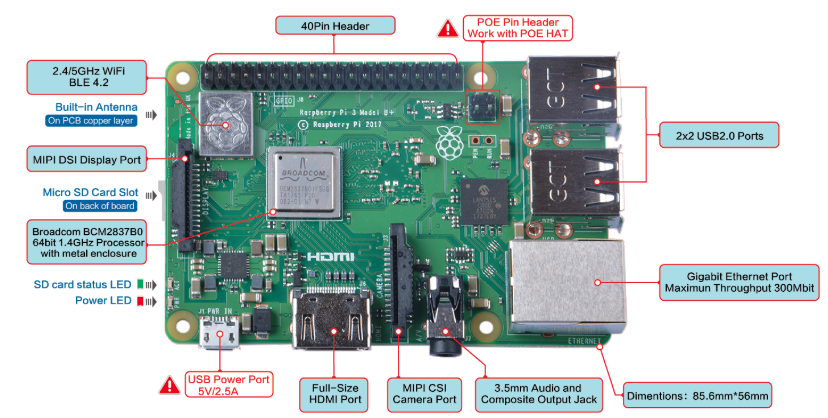
\includegraphics[width = .9\textwidth]{212.png}

\subsection{SunFounder Raspberry Pi Smart Video Car}

SunFounder is a technology company focused on Raspberry Pi and Arduino open source
community development. The Pi Car-S Robot is a smart car which work based on a Raspberry Pi.

The raspberry pi car comes with three sensor modules including ultrasonic obstacle avoidance, light follower, and line follower. The car robot has durable and shatterproof plate and new style Servo, the MAX torque of the clutch gear digital servo is up to 1.6KG[9]. It rotates from 0-180 degrees.

Python code is provided for the car, and users can also program and debug it with Dragit, a Snap-based graphical interface, by just simple dragging and dropping the code blocks for more complex functions. A user can learn the programming conveniently on how to control the car.

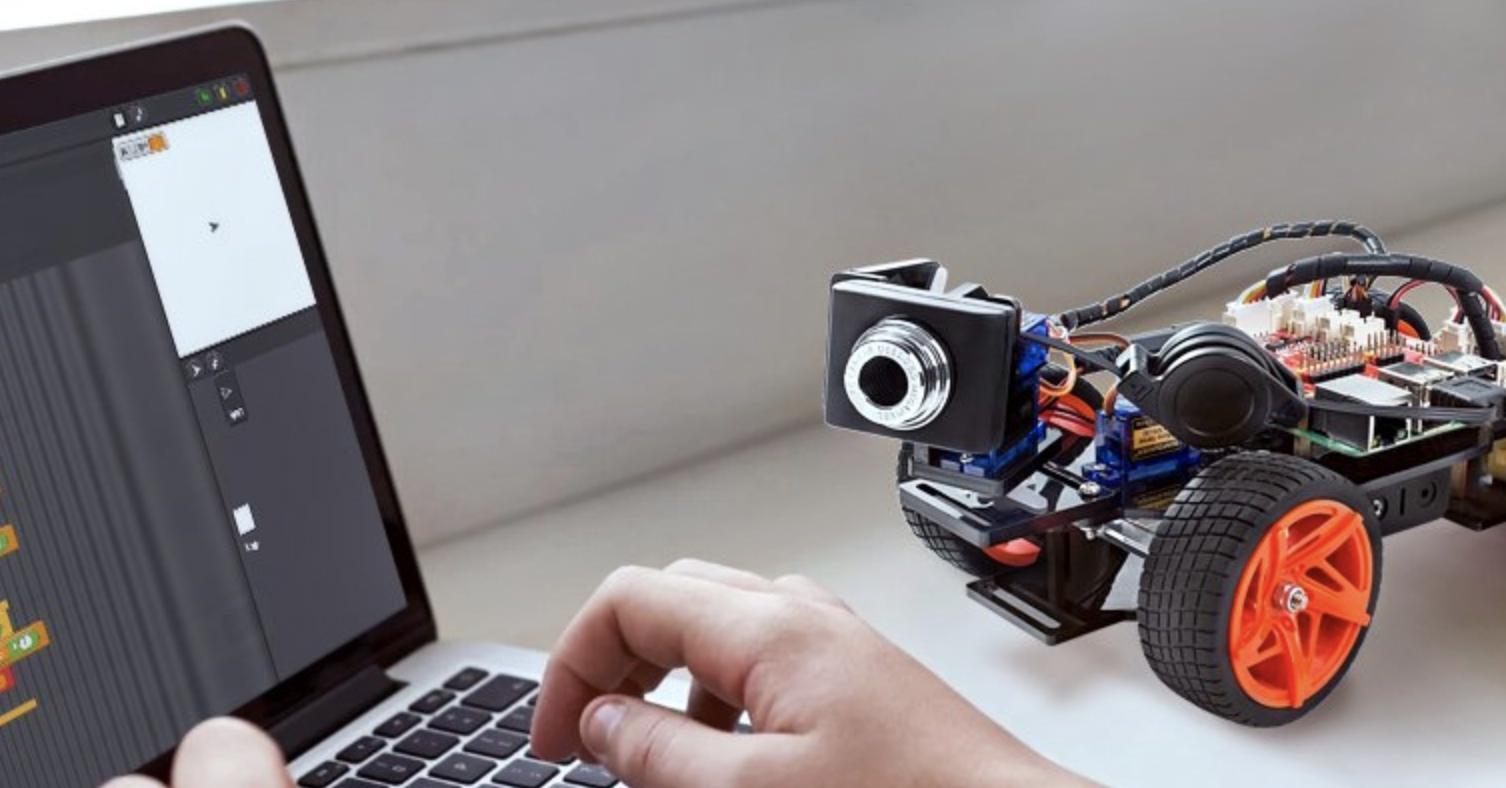
\includegraphics[width = .7\textwidth]{a.jpg}

\section{Robot Software and Operating System}
The following sections introduce the Robot software and operating system that used in this project. The version of ROS and ROS2 is under development and changes frequently these years.

\subsection{ROS}
Robot Operating System (ROS or ros) is robotics middleware (i.e. collection of software frameworks for robot software development). ROS is not an operating system. It is a set of software libraries and tools that help people build robot applications. From drivers to state-of-the-art algorithms, and with powerful developer tools and it’s all open source[11]. ROS is a software framework meant to allow people to write applications which operate robotic hardware. As its most fundamental level, it is an abstraction layer - offering hardware abstraction.  

Robotic middleware is a software infrastructure that is intended to provide convenient abstraction and communication paradigms for facilitating this multi-subsystem approach. In general, a robotics middleware would provide a common interface design so that no matter what hardware is producing the data, the results are distributed in a consistent manner[10].


Robot Operating System is mainly composed of 2 things[12]: \\
1. A core (middleware) with communication tools. \\
2. A set of plug and play libraries.

\subsection{ROS 2}
ROS2, which is a new version of ROS that is under heavy development. ROS2 is the next generation robot operating system, and is actively being developed to fully replace ROS in the near future. The goal of the ROS2 project is to adapt to previous changes, leveraging what is great about ROS and improving what is not[13]. 

A further reason to build ROS 2 is to take advantage of the opportunity to improve our user-facing APIs. A great deal of the ROS code that exists today is compatible with the client libraries as far back as the 0.4 “Mango Tango” release from February 2009. That’s great from the point of view of stability, but it also implies that we’re still living with API decisions that were made several years ago, some of which we know now to be not the best[14].

There some obvious differences between ROS and ROS2: \\
1. ROS1 is targeting Python 2, but ROS2 requires at least Python version 3.5. \\
2. Catkin make is gone: Catkin has been replaced by colcon. This new building system is in essence a universal building system for the ROS ecosystem. \\
3. ROS2 uses rclpy as Python client library which replace roscpp in ROS.

\subsection{Ubuntu}
Ubuntu is a complete Linux operating system, which is an open source Debian-based Linux distribution. Ubuntu is now the most used Linux operating system, both for desktops and servers.

Ubuntu is built on Debian's architecture and infrastructure, and comprises Linux server, desktop and discontinued phone and tablet operating system versions.[15] Ubuntu releases updated versions predictably every six months, and each release receives free support for nine months[16]. Downloading, installing, and using Ubuntu Linux doesn’t cost a penny. Installing Ubuntu does not need high-end system requirements. So it is a ideal operating system for Raspberry Pi, as the Raspberry Pi has limited memory CPU performance. 

Ubuntu is available in a number of different flavours, each coming with its own desktop environment. Ubuntu MATE takes the Ubuntu base operating system and adds the MATE Desktop. The MATE Desktop is one such implementation of a desktop environment and includes a file manager which can connect you to your local and networked files, a text editor, calculator, archive manager, image viewer, document viewer, system monitor and terminal[17]. And Ubuntu Mate offer specific downloading installing package for Raspberry Pi. This can be downloaded from the official site.

Furthermore, Ubuntu is also the recommended operating system in ROS. ROS offers more support for a few Ubuntu version. There is another operating system called Raspbian which is widely installed on Raspberry Pi. However, Raspbian is not well supported by ROS and it may occur many problems when installing ROS in Raspbian. Therefore, ubuntu is used in this experiment for Raspberry Pi as operating system.

\section{ROS Communication}

\subsection{Star Network Topology}
A star topology is a topology for a Local Area Network (LAN) in which all nodes are individually connected to a central connection point, like a hub or a switch. A star takes more cable than e.g. a bus, but the benefit is that if a cable fails, only one node will be brought down[18].

All traffic emanates from the hub of the star. The central site is in control of all the nodes attached to it. The central hub is usually a fast, self contained computer and is responsible for routing all traffic to other nodes. The main advantages of a star network is that one malfunctioning node does not affect the rest of the network. However this type of network can be prone to bottleneck and failure problems at the central site.

It is the most common network topology in real life, as it is easy to install, scalable and easy to troubleshoot. At the centre of the network sits the multifunctional wireless router providing the functionality of a wireless access point (WAP), a modem, a switch and a router.

Star network topology is also used in this experiment for testing message latency communicating in different devices with a center router.

The network graph is as follows:
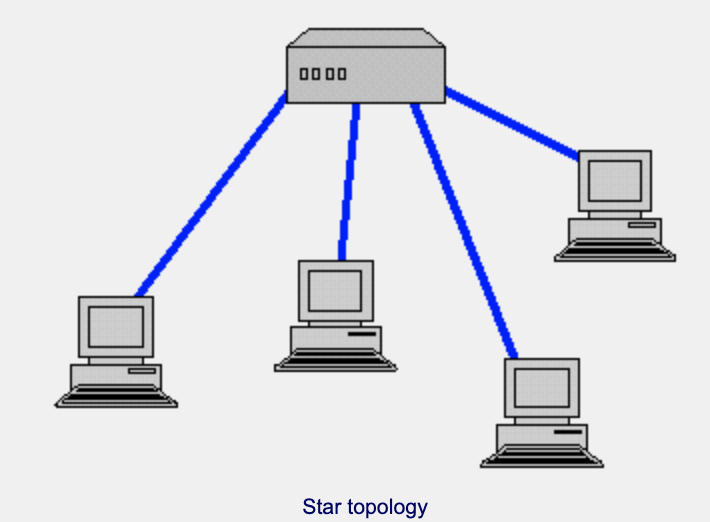
\includegraphics[width = .7\textwidth]{231.png}

\subsection{TCP and UDP}
Both TCP and UDP work on top of the IP (Internet Protocol). This is why there are terms such as TCP/IP or UDP/IP. In the OSI model, TCP and UDP are both "Transport Layer" Protocols[19]. Where TCP is a connection oriented protocol and UDP is a connectionless protocol.  

TCP and UDP are network protocols that are used to send data packets. These data packets are just bits of data that travel over the internet. When a user chat with his friends online, send an email, or send a page request through browser, he sends online data. This data is transferred in the form of tiny packets. While TCP and UDP are the most commonly used protocols, they aren’t the only ones used to transfer data packets. Another protocol that can be used is ICMP (Internet Control Message Protocol). However, most connections rely on either TCP or UDP.

There are three main differences between TCP and UDP[20]:

1. Reliability
TCP is more reliable since it manages message acknowledgment and retransmissions in case of lost parts. Thus there is absolutely no missing data. UDP does not ensure that communication has reached receiver since concepts of acknowledgment, time out and retransmission are not present.

2. Ordering
TCP transmissions are sent in a sequence and they are received in the same sequence. In the event of data segments arriving in wrong order, TCP reorders and delivers application. In the case of UDP, sent message sequence may not be maintained when it reaches receiving application. There is no way of predicting the order in which message will be received.

3. Connection
TCP is a heavy weight connection requiring three packets for a socket connection and handles congestion control and reliability. UDP is a lightweight transport layer designed atop an IP. There are no tracking connections or ordering of messages.

In this experiment ROS use TCP and ROS2 use UDP.

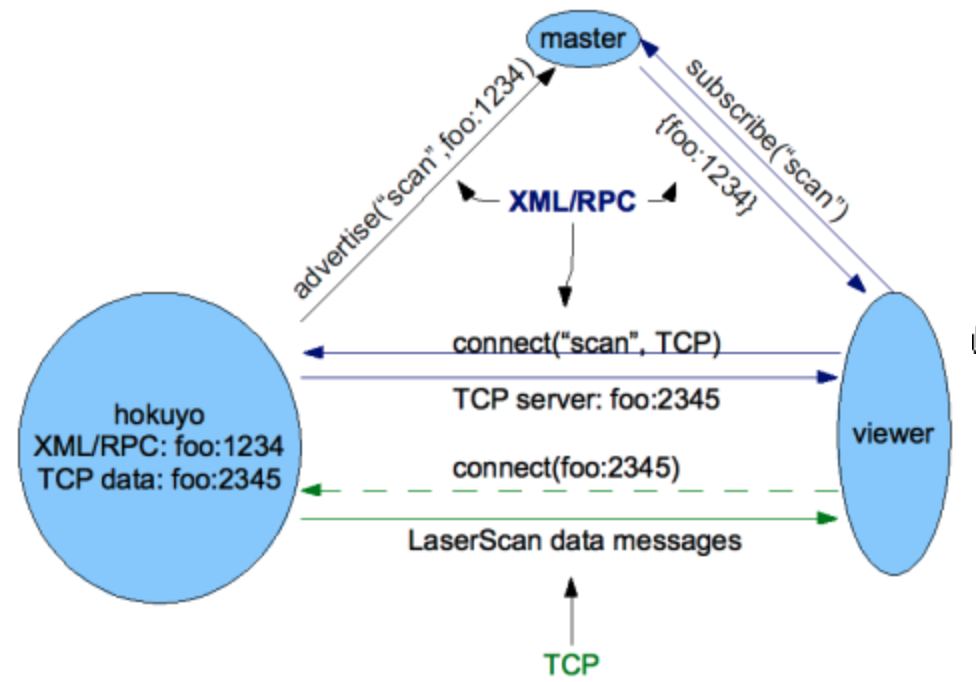
\includegraphics[width = .7\textwidth]{d.png}

%%%%%%%%%%%%%%%%%%%%%%%%%%%%%%%%%%%%%%%%%%%%%%%%%%%%%%%%%%%%%%%%%%%
\chapter{Installation and configuration}

\section{Ubuntu and ROS system installation}

ubuntu version bits
\subsection{Steps}
1. Down load the latest version image of Ubuntu with ROS in the ROS official website.

2. Write the image to Raspberry Pi by using SD card.

3. Start the ubuntu system with installed ROS and envonriment automatically. 

4. Type `roscore` to test whether ROS system exist.
\subsection{Issues and Solution}
Raspbian 10(buster) is not well supported by ROS system. There are some outdated dependencies which is needed in installing ROS. Therefore, there are many bugs and manually installation steps to solve when user want to install ROS in Raspbian operating system. Then the ubuntu is recommend operating system as official website said.


\section{Router network configuration}
1. Each Raspberry Pi should connect to the same LAN.

2. Assign static IP address to each Raspberry Pi for ssh remote control and management.

3. Using one computer to join this LAN for controlling the all Raspberry Pi.

4. Remote control other Raspberry Pi by ssh using `ssh {hostname}@{ip address}` with password.


\section{Communication between different ROS hosts}
\subsection{Change the host file}
1. each host configuration file list should be  
    `sudo vim /etc/hosts`
    
2. Add ip address and hostname in `/etc/hosts` file of your Raspberry Pi. Each ip address respond to one hostname which you give.
Example hosts file:

\begin{verbatim}
ff02::1 ip6-allnodes
ff02::2 ip6-allrouters

192.168.1.11 com1
192.168.1.12 com2
\end{verbatim}

\subsection{Talker and Listener}
Enter ROS system in every ubuntu system and ssh to com1. Then ping com1 and com2. If ping successfully meaning the network is fine, otherwise check the router and network problem.

The host name and ip address is respond to each Raspberry Pi, but the Master URI should be identical. Create a .sh file to export environment paths.
\begin{verbatim}
# /bin/sh
export ROS_HOSTNAME=com1
export ROS_IP=192.168.1.11
export ROS_MASTER_URI=http://com1:11311/
\end{verbatim}

Configure the file and execute this file in every Raspberry Pi host. Then run the talker and listener python file separatlly in different hosts to check if listener can receive messages from talker.

\subsection{Issues and Solution}
Make sure setting the ROS hostname and IP address correctly and must explicitly set it. Otherwise the listener cannot receive talker because the host cannot find it in the network. The Talker will send messages continuously but listener can not receive these messages.

Check the hostname and ip address setting can use:
\begin{verbatim}
`echo $ROS_HOSTNAME`
`echo $ROS_IP`
\end{verbatim}

%%%%%%%%%%%%%%%%%%%%%%%%%%%%%%%%%%%%%%%%%%%%%%%%%%%%%%%%%%%%%%%%%%%
\chapter{Experiment and Analysis}

\section{Experiment 1: Revising wifi router performance experiment}
\textbf{Objective} \\
This experiment investigates the performance in different frequency of message passing by using Wi-Fi network connection in a router.  This experiment was executed by Issac in the previous and my aim is execute this experiment to compare it with the previous one.

\textbf{Rationale} \\
In order to acquire a detailed understanding of the performance characteristics of ROS’ communication channels, this experiment use two ROS hosts to commnunicate with each other and get the message latency results in different message frequency. I reproduced Issac's experiment to see what is the difference between my experiment and the previous one then analyze the reason to cause these differences.

\textbf{Procedure} \\
1. Install ROS and ubuntu in Raspberry Pi 3B+ \\
2. Sending message and receive message between two hosts to test communication. \\
3. Sending 10HZ message and test message latency. \\
4. Run the code which send timestamped messages from the sender host to the echoer host. The sender will receive the message and then record message id into a file. The code is run 3 times with a range of message frequencies from 1hz to 2000Hz to obtain averaged results for each message frequency.

\textbf{Hardware Configuration} \\
2 Raspberry Pi 3B+ \\
TP-Link 150M router

\textbf{Software Configuration} \\
Ubuntu 16.04 \\
ROS Kinetic 

\textbf{Hypothesis} \\
1. The latency should be not regular(explain) due to the wifi connection is not stable. \\
2. Different message frequency may perform different latency due to the wifi environment.

\textbf{Results} \\
The data which I collect and plot is as follows, the left one is mine and the right one is Issac's experiment graph.

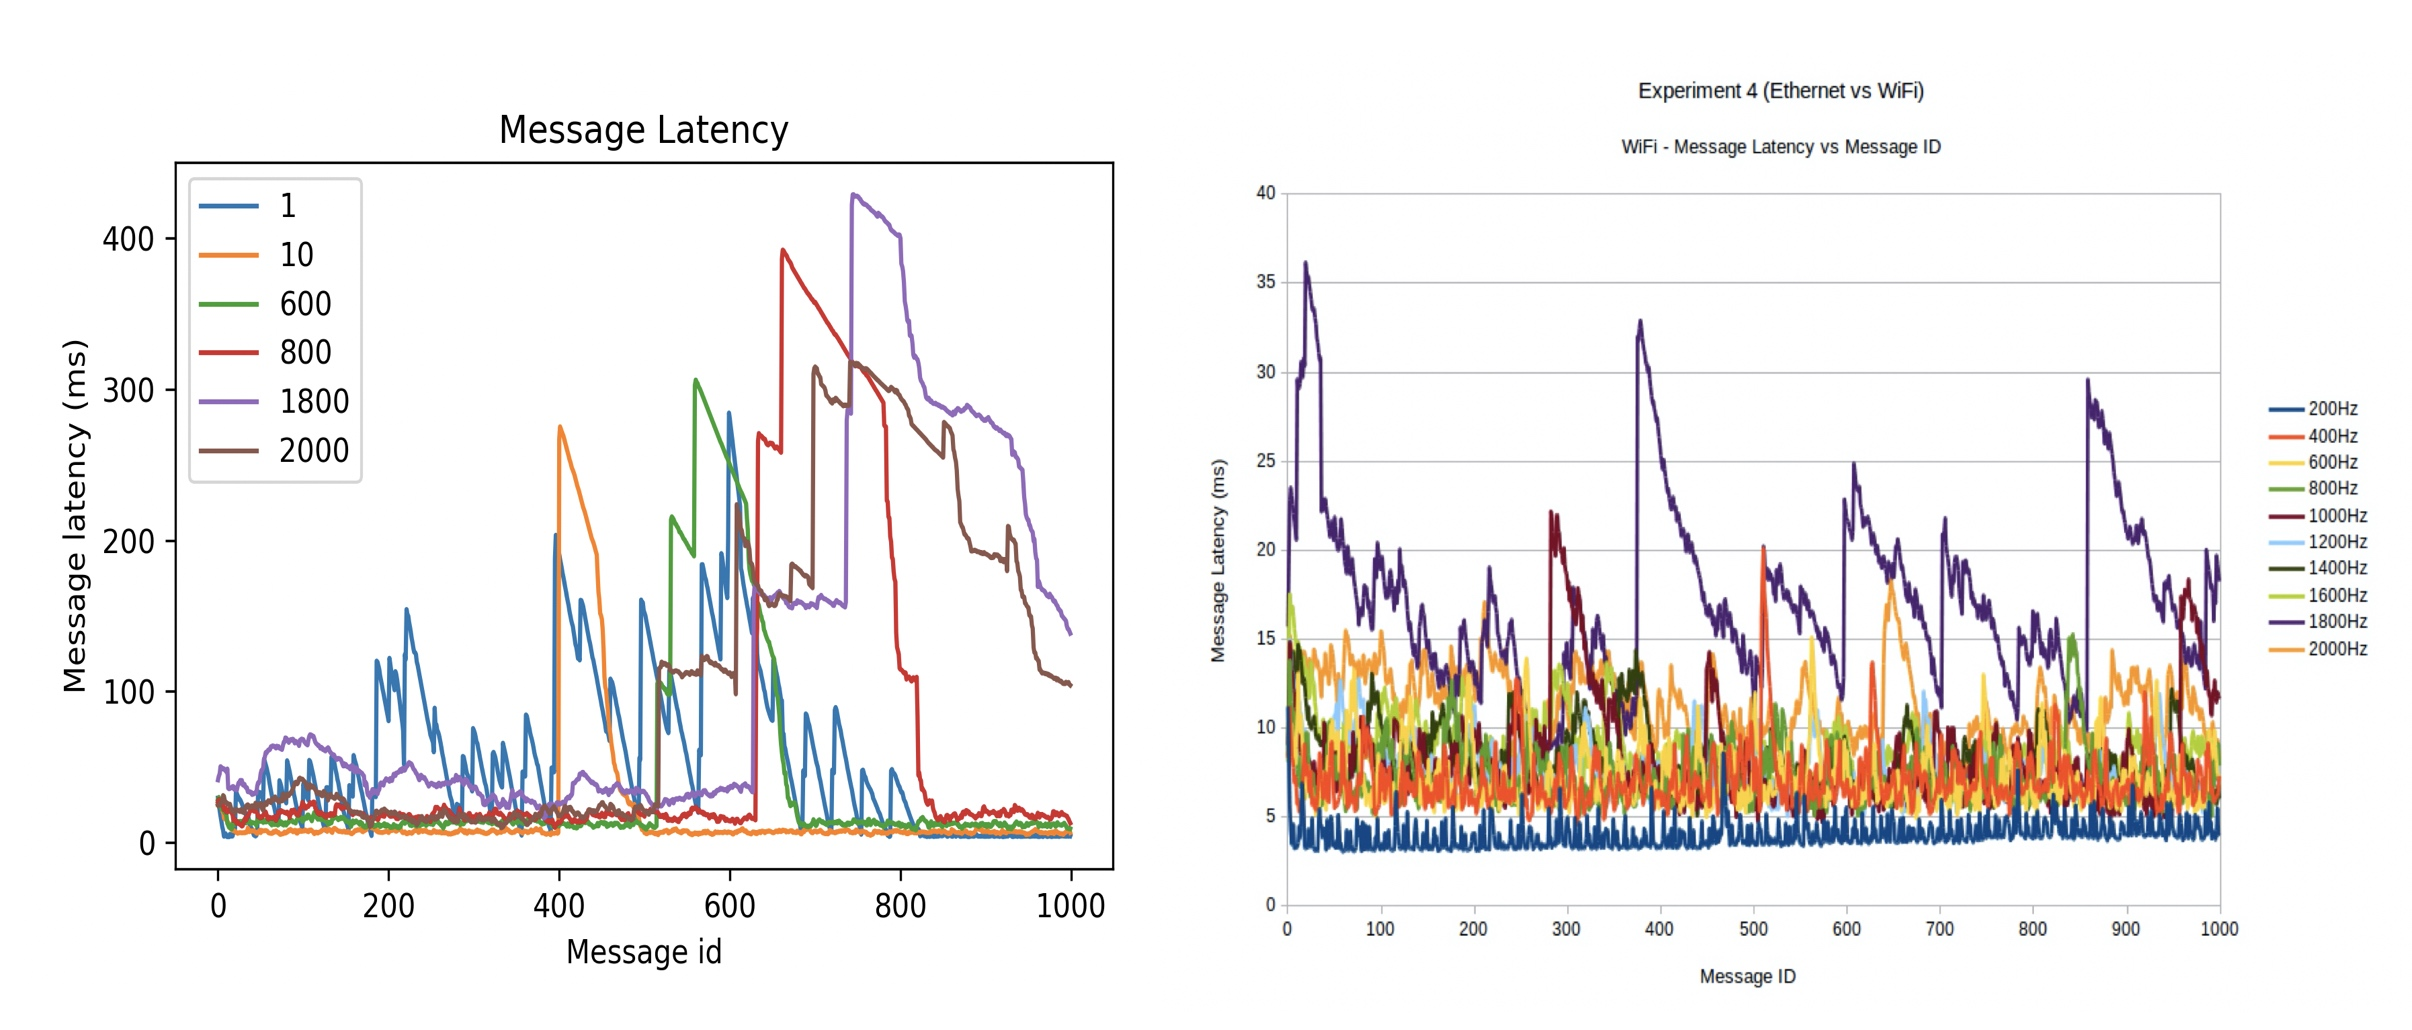
\includegraphics[width = 1\textwidth]{compare_issac.jpg}

\textbf{Conclusion} \\
The previous experiment by Issac shows lower latency and I think that is due to the different hardware and some other environment factors.

The message latency is not regular and different frequency can perform relatively different latency. Wifi connection can be different in different time so that is why the latency is obvious in specific time period.


\clearpage
 3
\clearpage
 4
\clearpage
 5
\clearpage
 6


%%%%%%%%%%%%%%%%%%%%%%%%%%%%%%%%%%%%%%%%%%%%%%%%%%%%%%%%%%%%%%%%%%%
\chapter{Conclusion}\label{conclusion}
1



\clearpage
2



\appendix % first appendix
%%%%%%%%%%%%%%%%%%%%%%%%%%%%%%%%%%%%%%%%%%%%%%%%%%%%%%%%%%%%%%%%%%%
\chapter{First appendix}

\section{Section of first appendix}

%%%%%%%%%%%%%%%%%%%%%%%%%%%%%%%%%%%%%%%%%%%%%%%%%%%%%%%%%%%%%%%%%%%
\chapter{Second appendix}

%%%%%%%%%%%%%%%%%%%%%%%%%%%%%%%%%%%%%%%%%%%%%%%%%%%%%%%%%%%%%%%%%%%
% it is fine to change the bibliography style if you want
\bibliographystyle{plain}
\bibliography{mproj}
[1] Sandra May. What Is Robotics?  \url{https://www.nasa.gov/audience/forstudents/k-4/stories/nasa-knows/what_is_robotics_k4.html}. Nov. 9, 2009

[2] B. Bauml and G. Hirzinger. Agile Robot Development (aRD): A Pragmatic Approach to Robotic Software. In 2006 IEEE/RSJ International Conference on Intelligent Robots and Systems, pages 3741–3748, Oct 2006.

[3] Avinash Gautam and Sudeept Mohan. A review of research in multi-robot systems. In 2012 IEEE 7th International Conference on Industrial and Information Systems (ICIIS), pages 1–5. IEEE, Aug 2012.

[4] Pedro U. Lima and Luis M. Cust´odio. Multi-Robot Systems. In Innovations in Robot Mobility and Control, pages 1–64. Springer, Berlin, Heidelberg, Aug 2005.

[5] Zhi Yan, Nicolas Jouandeau, and Arab Ali Cherif. International Journal of Advanced Robotic Systems, 10(12):399, 2013.

[6] Deborah Estrin, David Culler, Kris Pister, and Gaurav Sukhatme. Connecting the physical world with pervasive networks. IEEE pervasive computing, 1(1):62–63, 2002.

[7] Cellan-Jones. A£15 computer to inspire young programmers. BBC news. 5 May 2011

[8] Gibbs, Samuel. Raspberry Pi becomes best selling British computer. The Guardian. Retrieved 28 December 2016.

[9] SunFounder PiCar-S Kit V2.0 page. \url{https://www.sunfounder.com/picar-s-kit.html}. 

[10] Isaac Jordan. Robotic Middleware. \url{https://github.com/Sheepzez/ros-multirobot-evaluation/tree/master/experiments/message_latency/no_ echo_delay_no_disk_write}. 2017-03-18.

[11] ROS Melodic Morenia. \url{wiki.ros.org}. Retrieved 10 June 2018.

[12] The Robotics Back-End Home page. \url{https://roboticsbackend.com/what-is-ros}. 2019

[13] ROS2 Overview Home page. \url{https://index.ros.org/doc/ros2/}

[14]  Brian Gerkey. Why ROS 2?. \url{http://design.ros2.org/articles/why_ros2.html}

[15]"Ubuntu and Debian". Ubuntu.com. Canonical Ltd. Retrieved 14 December 2013.

[16]"Ubuntu and Debian". Ubuntu.com. Canonical Ltd. Retrieved 14 December 2013.

[17] What is Ubuntu MATE?. Ubuntu MATE Team. \url{https://ubuntu-mate.org/what-is-ubuntu-mate/}. 2019 

[18] Star topology. \url{http://www.telecomabc.com/s/star.html}. 2015



[6] "Linux 2 6 38". Linux Kernel Newbies.

[8] "Zero WH: Pre-soldered headers and what to do with them". Raspberry Pi Foundation. Retrieved 12 January 2018.

[9] "FrontPage - Raspbian". \url{www.raspbian.org}. Retrieved 2016-04-04.

[10] "Introducing PIXEL - Raspberry Pi". Raspberry Pi. 2016-09-28. Retrieved 2017-01-07.


[19] "Communication Networks/TCP and UDP Protocols". \url{https://en.wikibooks.org/wiki/Communication_Networks/TCP_and_UDP_Protocols}.

[20] "What’s the Difference Between TCP and UDP?". \url{https://www.howtogeek.com/190014/htg-explains-what-is-the-difference-between-tcp-and-udp/}.

[21] "Star topology". Cisco Networking Academy 2014.

[22] "Mesh topology". \url{https://www.computerhope.com/jargon/m/mesh.htm}.

[23] "Open Mesh". \url{https://www.openmesh.com/datto-networking}.




[27] "Changes between ROS 1 and ROS 2". \url{http://design.ros2.org/articles/changes.html}.

\end{document}
